\section{Použití trezoru}
První nasazení trezoru na akci pořádané Robotárnou \parencite{robotarna} proběhlo na pří\-měst\-ském robotickém táboře v~srpnu roku 2019.
Jednalo se o~první variantu trezoru, která kdy spatřila světlo světa (viz kapitola \ref{E1-vyvoj}). 
Tábor trval pět dní a~děti dostaly první tři dny na stavbu mechaniky a~poslední dva dny 
se~programovalo. 

Trezor tehdy sklidil úspěch, a~tak započal vývoj dalších verzí, které už byly specializovanější 
(viz kapitoly \ref{E2-vyvoj} a~\ref{E3-vyvoj}) a~přidal se i~vývoj mechanických
variant (viz kapitola \ref{M3}).

V~průběhu vývoje se trezor použil na řadě akcí:

\begin{itemize}
    \item Příměstský tábor 2019 
    \item Robotický kroužek 2019/20
    \item Zážitková stavební akce 2020  %netušim jak to kulantně nazvat ale byla to akce pro decka na nějaký pobočce 
                                        %myslim že v Bityšce ale nebyl jsem tam tak si nejsem jistej
    \item Skautská akce 2020
    \item Akce instruktorů 2020
    \item Robotický tábor 2020
\end{itemize}
Celkově BlackBox v~nějaké verzi použilo alespoň 110 lidí, pravděpodobně ale víc, přesné číslo bohužel neznám.

\paragraph{Trezor ve volnočasových kurzech robotiky}
Další používání trezoru pro\-bí\-ha\-lo ve volnočasovém kurzu robotiky, který jsem spoluvedl, a~účastníci v~něm stavěli mechanickou 
variantu.
Protože účastníci kurzu byli vetšinou již docela zkušení, jednalo se u~nimi téměř jen o~\uv{rozcvičku}, 
kterou měli za několik kroužků hotovou a~následovala stavba elektronického BlackBoxu. 

Bohužel kvůli pandemickým opatřením si ne všichni účastníci stihli BlackBox postavit a~vůbec jsme se nedostali k~programování, 
natož aby jsme si s~trezorem zorganizovali nějakou herní akci, jak bylo dříve v~plánu.

\paragraph{Trpasličí trezor}
Chvíli po té, co vznikl mechanický BlackBox (viz kapitola \ref{M3}), proběhla první akce s~BlackBoxem, která nebyla pod taktovkou Robotárny. 
Zároveň to byla také první akce, na které se trezor nestavěl a~jen se využíval.

Protože na akci byly menší děti, byl trezor místo klasické číselné stupnice  vybaven obrázkovým kódem, jak je vidět na obrázku \obr{fig:M3-trpaslici}. %todo co se tam s tím trezorem dělalo 

Toto však byla poslední akce, která se stihla uskutečnit před započetím pandemických opatření.

\begin{figure}[htbp]
    \centering
    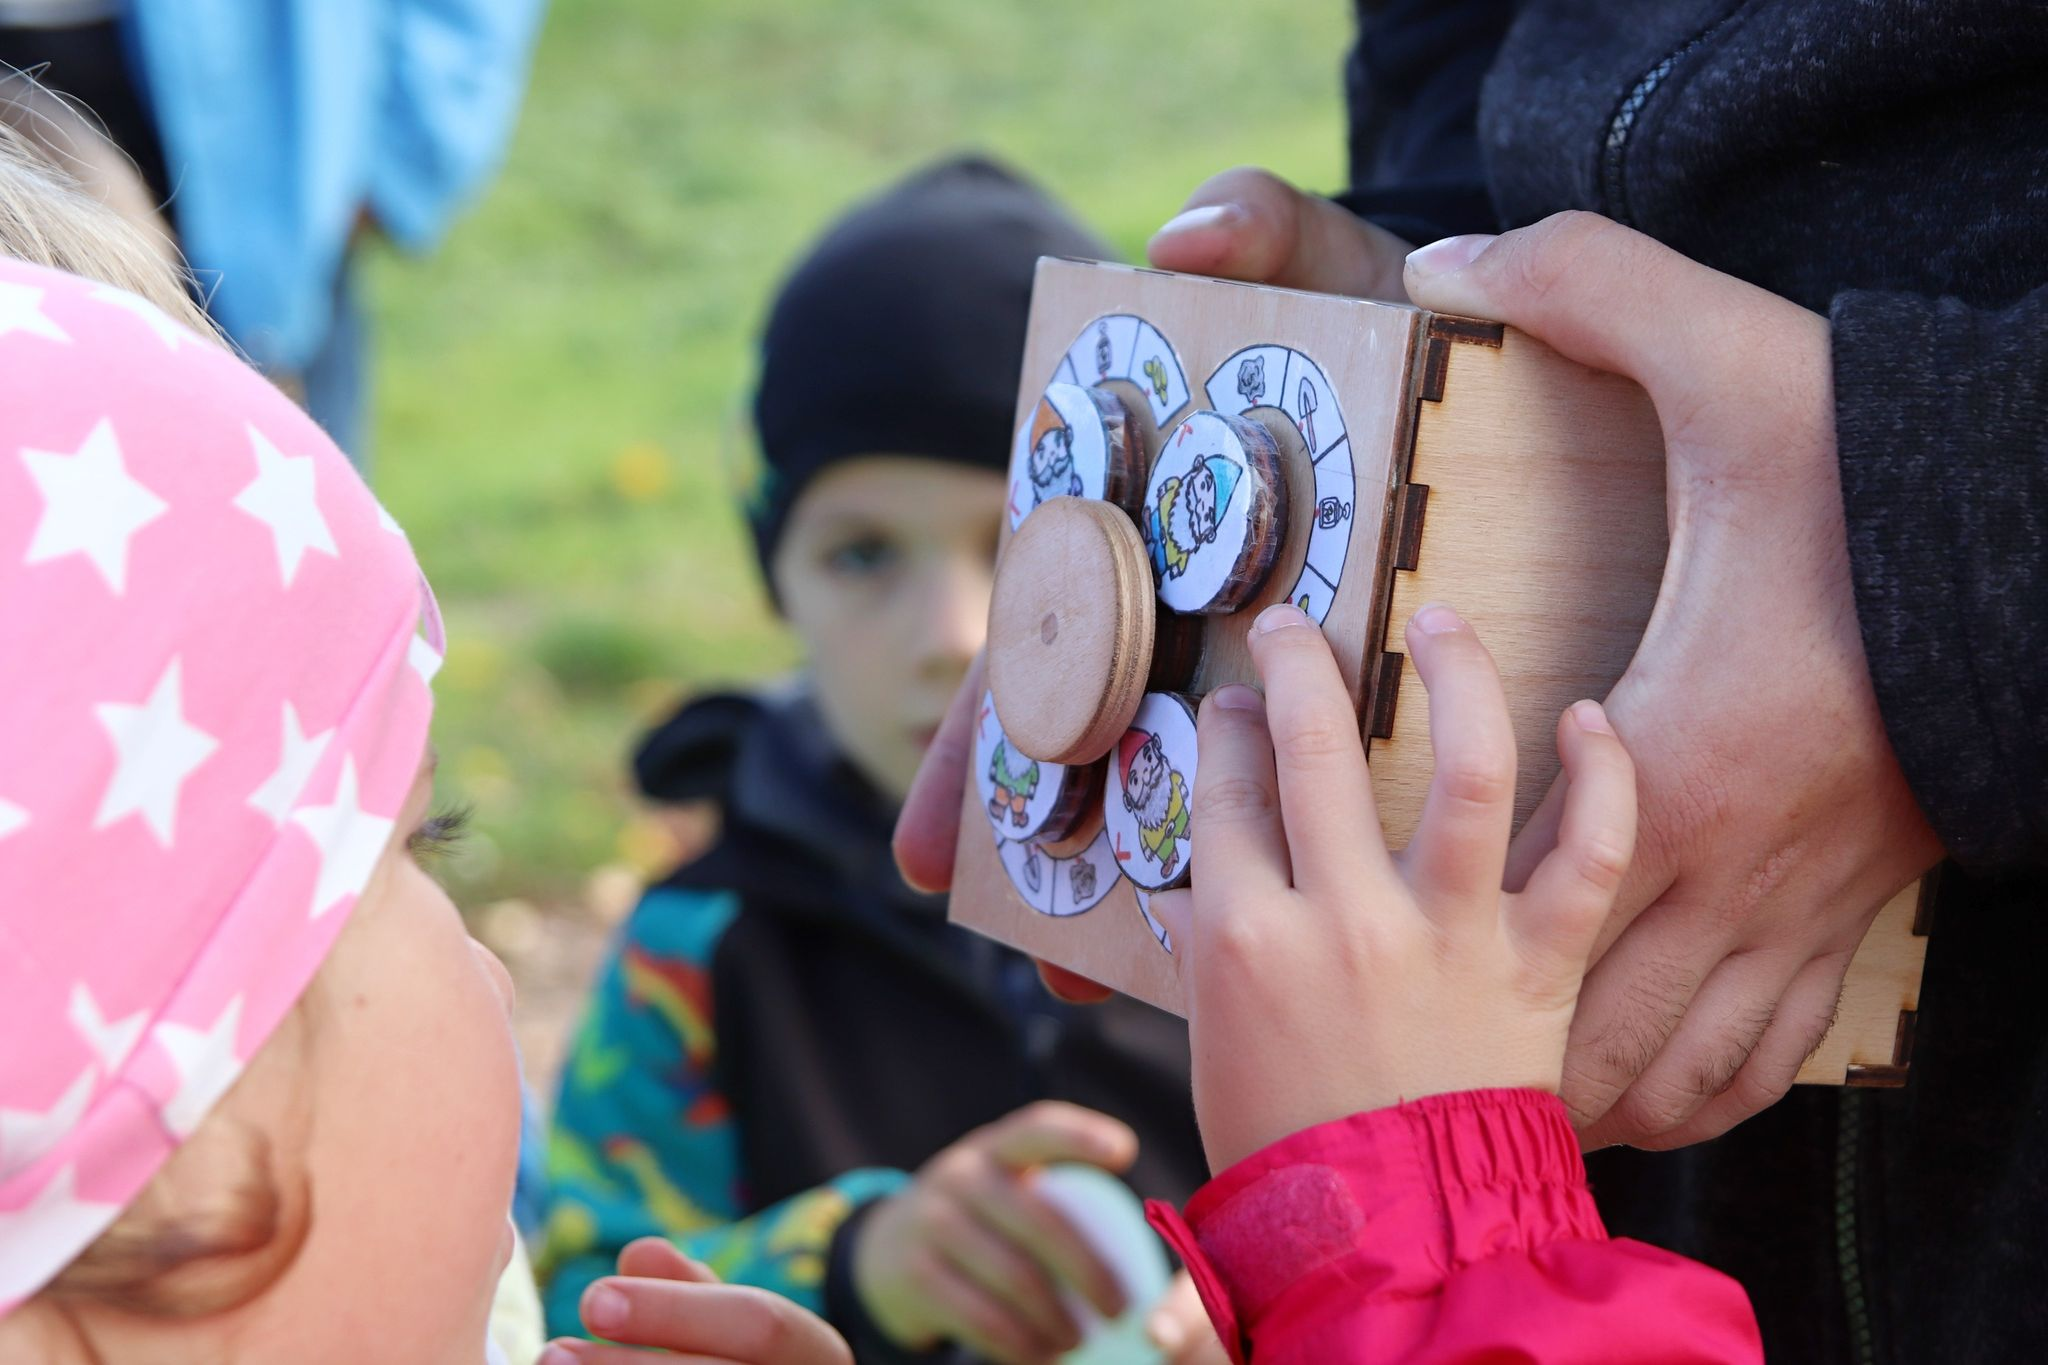
\includegraphics[width=0.9\textwidth]{kapitoly/obrazky/M3/trpaslici.png}
    \caption{Trpasličí trezor}
    \label{fig:M3-trpaslici}
\end{figure}